\documentclass[preprint,12pt]{elsarticle}

\usepackage{amsmath,amssymb,amsthm,mathtools}
\usepackage{booktabs}
\usepackage{tabularx}
\usepackage{array}
\usepackage{microtype}
\usepackage{xcolor}
\usepackage{tikz}
\usepackage{pgfplots}
\usepackage{enumitem}
\usepackage{xurl}
\usepackage{hyperref}
\usetikzlibrary{arrows.meta,positioning}
\pgfplotsset{compat=1.18}
\hypersetup{hidelinks}

\journal{Journal of Information Security and Applications}

\newtheorem{definition}{Definition}
\newtheorem{theorem}{Theorem}
\newtheorem{proposition}{Proposition}
\newtheorem{corollary}{Corollary}
\newtheorem{lemma}{Lemma}
\newcommand{\Cl}{\operatorname{Cl}}
\newcommand{\UDC}{\mathsf{UDC}}
\newcommand{\Derived}{\mathsf{Derived}}
\newcommand{\Cost}{\operatorname{cost}}
\newcommand{\powerset}{\mathcal{P}}
\newcolumntype{Y}{>{\raggedright\arraybackslash}X}
\newcolumntype{R}[1]{>{\raggedright\arraybackslash}p{#1}}

\begin{document}

\begin{frontmatter}

\title{Credential Exposure Threshold Spectra for Distributed Password Derivation}

\author{Yuanyi Zhang}
\address{Independent Researcher}

\begin{abstract}
Threshold sharing and distributed pseudorandom functions are commonly assessed
by asking how many parties must be compromised before a master secret becomes
available.  For deterministic password derivation, this single threshold can
miss a different failure: a compromised endpoint may keep the master secret
hidden while using an over-broad evaluation interface to obtain many
credential outputs.  We define a finite capability-closure model that computes
unrestricted derivation capability (UDC) and context-indexed credential
exposure from the same
compromise and approval state.  Its quantitative output, the credential
exposure threshold spectrum, gives the minimum number or monotone set cost of
deployment domains needed to expose at least $k$ unauthorized credential
contexts under an approval budget $q$.  We prove UDC dominance, show why a
UDC-only analysis is incomplete below its threshold, establish monotonicity
and UDC bounds for the spectrum, and derive an exact exposure formula for
projection-bound authorization tickets.  A reference analyzer accepts an
arbitrary monotone compromise-set cost and produces minimal witnesses.  We
also instantiate a complete two-server scoped key-derivation path with
RFC~9497 POPRF and signed tickets.  Over 32 contexts, complete binding accepts
one context, service/account-only binding accepts eight, and wildcard binding
accepts all 32.  Their thresholds are respectively two throughout; one for
$k\le7$ and two thereafter; and one for $k\le31$ and two for $k=32$.  The local cryptographic path
costs 1.15~ms median, excluding network and human approval delay.
A temporal TLA+ model exhaustively checks ticket issue, expiry, revocation,
replay, generation change, UDC dominance, and scope confinement, with a
positive model and five fault controls.  The contribution is a
credential-specific analysis and metric, not a new sharing, PRF, token, or
attack-graph primitive.
\end{abstract}

\begin{keyword}
password derivation \sep distributed pseudorandom function \sep threshold
cryptography \sep authorization amplification \sep capability analysis
\sep credential exposure
\end{keyword}

\end{frontmatter}

\section{Introduction}

Distributed trust is attractive for credential recovery and derivation.
Shamir sharing makes a secret reconstructible only by a qualified set
\cite{shamir1979}; distributed pseudorandom functions (DPRFs) let qualified
parties evaluate a keyed function without reconstructing the key
\cite{naor1999dprf}.  Recent systems apply related techniques to password
hardening, multi-factor key derivation, distributed key management, and secret
recovery \cite{everspaugh2015pythia,jarecki2017toppss,nair2023mfkdf,
geihs2024lakey,connell2024svr3}.  Their cryptographic access structure is only
one part of the deployed security boundary.  An endpoint may hold a share, a
network-call credential, or authority to trigger honest infrastructure.  The
number of physical or administrative domains that an attacker must compromise
can therefore be smaller than the nominal share threshold.

Even a correctly deployed DPRF creates a second question.  Its security
definition controls what is learned from a bounded set of legitimate
evaluations; it does not decide which inputs the application should authorize.
If one ticket intended for account $c$ can be replayed for accounts
$c_1,\ldots,c_n$, the master key can remain unavailable while all corresponding
passwords become computable.  A binary question---``is unrestricted
derivation authority available?''---does not represent this partial but
operationally serious exposure.  Root-Key recovery is one common way to obtain
that authority, but it is not the only one.

Generic protection-system safety, attack graphs, capability safety, permission
expansion, and least-privilege authorization already study closely related
ideas \cite{hru1976,ou2005mulval,wang2006hardening,
maffeis2010capabilities,lee2021polyscope,cao2024leastprivilege}.  Consequently,
fixed-point reachability, minimum-cost compromise, and context-bound tokens are
not new contributions here.  The research question is narrower:

\begin{quote}
How can a deterministic credential-derivation deployment jointly report (i)
access to its UDC and (ii) the number of credential contexts made
derivable by compromised domains and scoped approvals?
\end{quote}

We answer with a dual-output closure and a credential exposure threshold
spectrum (CETS).  Rather than replace the UDC threshold, CETS resolves it into
a curve indexed by unauthorized output cardinality and approval budget.  This
immediately distinguishes a two-domain UDC threshold with exact per-context
authorization from a deployment with the same UDC threshold but a one-domain
path to most credential outputs.

The contributions are:

\begin{enumerate}[leftmargin=*,itemsep=3pt]
\item A finite semantics that derives UDC reachability $M_R(X,T)$ and the
  context-indexed output set $E_R(X,T)$ from one least fixed point over
  compromised deployment domains $X$ and attacker-observed approvals $T$.
\item CETS, including cardinality and general monotone set-cost forms,
  UDC-dominance and UDC-only-incompleteness results, monotonicity, and a
  UDC-threshold bound.
\item An exact projection-exposure identity and closed-form approval-budget
  profile for tickets that bind only selected context fields.
\item A small executable analyzer, a complete two-server RFC~9497 POPRF scoped
  key-derivation reference protocol with signed tickets, 24 automated tests, local
  measurements, and a temporal TLA+ model with positive and negative controls.
\end{enumerate}

The paper makes no new-primitive claim.  It does not propose a new Shamir
scheme, DPRF, OPRF, constrained PRF, capability token, or generic attack-graph
algorithm.  It also does not infer vulnerabilities in cited systems without a
faithful protocol encoding.

\section{Published foundations and novelty boundary}

\subsection{Access reachability and authority}

Harrison, Ruzzo, and Ullman formalized the safety question of whether a subject
can acquire a right \cite{hru1976}.  MulVAL uses Datalog rules for multihost,
multistage vulnerability analysis and produces attack explanations
\cite{ou2005mulval}.  Attack-graph research also optimizes compromise or
hardening cost \cite{wang2006hardening}.  These results establish both Horn-like
reachability and cost-based analysis as prior art.

Object-capability research distinguishes possession of a reference from the
authority reachable through program execution and formalizes authority safety
\cite{maffeis2010capabilities}.  PolyScope composes Android policies and system
configuration to compute permission expansion and authorized attack operations
\cite{lee2021polyscope}.  Stateful least-privilege authorization attenuates
tokens using action history to limit misuse after theft
\cite{cao2024leastprivilege}.  Our use of ``amplification'' is therefore not a
claim to a new general security principle.  We specialize the output dimension
to deterministic credentials and connect it to a Root-derived hierarchy.

\subsection{Scoped and distributed pseudorandom evaluation}

Constrained PRFs allow a derived key to evaluate only inputs satisfying a
constraint \cite{boneh2013constrained}.  Macaroons attach contextual caveats to
delegated authorization \cite{birgisson2014macaroons}.  These works establish
cryptographic input constraints and context-scoped capabilities; binding a
ticket to a complete context is a repair pattern rather than our primitive.

Pythia provides a verifiable partially oblivious PRF service for password
hardening and supports key rotation \cite{everspaugh2015pythia}.  TOPPSS uses a
threshold OPRF for password-protected secret sharing
\cite{jarecki2017toppss}.  LaKey studies efficient lattice DPRFs for scalable
distributed key derivation \cite{geihs2024lakey}.  These publications preclude
claims that remotely evaluated password-related PRFs, threshold OPRFs, hidden
master keys, or DPRF-based key derivation are new here.

\subsection{Recovery and deployment domains}

SafetyPin distributes encrypted-backup recovery across many HSMs and evaluates
the cost of large-scale compromise \cite{dauterman2020safetypin}.  MFKDF derives
keys from multiple factors and supports threshold recovery
\cite{nair2023mfkdf}; later analysis demonstrates why state integrity and exact
cryptographic specification matter \cite{scarlata2024mfkdf}.  SVR3 deploys
secret recovery across heterogeneous enclaves and cloud providers
\cite{connell2024svr3}.  Flock addresses how applications can deploy distinct
trust domains on demand \cite{kaviani2024flock}.  These systems motivate
deployment-domain analysis, but their stated evaluation objectives are not an
approval-budget-indexed spectrum of deterministic credential outputs.

Table~\ref{tab:boundary} states the boundary without classifying any published
system as insecure.

\begin{table}[t]
\centering
\caption{Published foundations and the narrower question studied here.}
\label{tab:boundary}
\small
\begin{tabularx}{\textwidth}{R{28mm} Y Y}
\toprule
Published line & Established analysis object & Object added in this paper \\
\midrule
HRU; MulVAL; attack graphs
  & Right/capability reachability and attack cost
  & Credential-output cardinality under an approval budget \\
Capability safety; PolyScope
  & Reachable authority, permission expansion, attack operations
  & Joint UDC/output signature for deterministic derivation \\
Constrained PRFs; Macaroons
  & Cryptographic constraints and contextual authorization
  & Exact diagnosis of collisions in a concrete context projection \\
Pythia; TOPPSS; LaKey
  & Password-related PRF services, threshold OPRF, distributed derivation
  & Spectrum below and up to a UDC threshold \\
SafetyPin; MFKDF; SVR3; Flock
  & Recovery, factor composition, and distributed trust deployment
  & Explicit composition of deployment-domain and callable-output exposure \\
\bottomrule
\end{tabularx}
\end{table}

\subsection{Why the object is not ordinary target-node counting}

An attack graph can encode each $\Derived(c)$ as a target node, and an existing
graph engine can be used to compute the closure in this paper.  CETS does not
claim otherwise.  Merely counting reachable target nodes, however, does not
define the quantity studied here.  Four additional structures are required.
First, the state is indexed by an attacker-observed approval set $T$ under an
explicit budget $q$.  Second, the security loss is the unauthorized set
$E_R(X,T)\setminus T$, rather than all reachable outputs; an approved password
is not counted as its own authorization failure.  Third, the distinguished
UDC dominates every credential target and therefore supplies a
global upper bound on the spectrum.  Fourth, a verifier that checks a context
projection induces equivalence classes whose sizes determine both single- and
multi-ticket spill.  These choices yield a two-parameter curve
$(k,q)\mapsto(\tau_E,\rho_E)$, not a new reachability algorithm.  A generic
attack-graph or Datalog implementation can serve as the backend only after
these credential-specific semantics and objectives have been supplied.

\section{System and threat model}

\subsection{Entities and contexts}

Let $D$ be a finite set of compromise domains.  A domain is an operational
failure boundary such as a managed endpoint, removable medium, approval
service, network evaluator, administrative account, or colocated group of
servers.  Multiple machines controlled by one administrative principal may be
one domain; machines do not become independent merely because they have
different addresses.

Let $C$ be a finite set of canonical credential contexts.  A context can
contain, for example,

\[
c=(\mathit{serviceID},\mathit{accountID},\mathit{lineage},
   \mathit{rootGeneration},\mathit{policyID}).
\]

Canonicalization is part of the model: field order, encoding, missing values,
and version semantics must be unambiguous.  We use a bounded $C$ because the
analyzer enumerates contexts; this represents a configured vault or a finite
test universe, not all possible future identifiers.

Let $K$ be a finite set of symbolic capabilities.  Examples include raw shares,
request tokens, approvals, partial evaluations, $\Derived(c)$, and $\UDC$.
The distinguished \emph{unrestricted derivation capability} $\UDC$ denotes
authority sufficient to compute every $\Derived(c)$ for $c\in C$ using the
public derivation procedure.  It is an authority abstraction, not necessarily
a single materialized key.  A reconstructed Root Key can imply $\UDC$; in the
reference POPRF case, $\UDC$ requires the endpoint-held input $x$ together
with either the approval-signing authority (while the evaluators remain honest
online participants) or both evaluator keys.
Accordingly, a well-formed rule set includes
$\{\UDC\}\rightarrow\Derived(c)$ for every $c\in C$.  ``Root capability'' is
used only when discussing the Root-Key instance of this more general object.
Let $R$ contain monotone rules whose consequences are automatically
exercisable by the attacker after their premises are available.  A human
decision is not automatic unless the threat model explicitly places that
decision under attacker control.

\subsection{Attacker and approvals}

The attacker compromises a set $X\subseteq D$ and obtains the capabilities
resident in those domains.  The set $T\subseteq C$ denotes legitimate approval
tickets that the attacker can observe, steal, or invoke within the analyzed
session.  It does \emph{not} mean all approvals issued elsewhere.  A ticket may
be modeled as an exact capability $\mathsf{Approval}(c)$ or by the fields that
its verifier actually checks.

The attacker can exercise every automatic rule, choose derivation requests,
and run the public derivation algorithm after obtaining $\UDC$.
In the reference POPRF experiment, the stable client input $x$ is resident at
the modeled endpoint and is available after endpoint compromise for every
configured context; it is not a separate authorization domain.
Cryptographic primitives are idealized: shares are not forged,
MACs and signatures are not broken, and a reviewed DPRF reveals only outputs
allowed by its application interface.  Availability attacks, social
engineering, side channels, and compromise during legitimate plaintext use are
outside the current model.

\subsection{Security goals}

The configured deployment has an intended minimum compromise-domain threshold
$t_{\mathrm{cfg}}$.  Two distinct goals are checked:

\begin{enumerate}[leftmargin=*]
\item \emph{UDC-threshold preservation}: no $X$ with
  $|X|<t_{\mathrm{cfg}}$ reaches $\UDC$.
\item \emph{authorized-context non-amplification}: for protected $X$ and a
  bounded approval set $T$, derivable credential contexts remain within $T$.
\end{enumerate}

An approved password can be visible to a compromised endpoint.  The second
goal only states that this approval does not become authority for additional
credential contexts.

\section{Joint capability semantics}

\begin{definition}[Initial capability set]
$C_0(X,T)$ is the union of public capabilities, the capabilities stored in
compromised domains $X$, and the modeled approval capabilities corresponding
to attacker-observed tickets $T$.
\end{definition}

\begin{definition}[Capability closure]
For monotone rule set $R$, define
\begin{equation}
\Cl_R(X,T)=\operatorname{lfp}
\left(S\mapsto C_0(X,T)\cup\operatorname{consequences}_R(S)\right).
\label{eq:closure}
\end{equation}
Because $K$ is finite and rules only add capabilities, iteration from
$C_0(X,T)$ reaches the unique least fixed point in at most $|K|$ additions.
\end{definition}

\begin{definition}[Dual output]
The UDC predicate and credential-exposure map are
\begin{align}
M_R(X,T)&=1 \quad\Longleftrightarrow\quad \UDC\in\Cl_R(X,T),\\
E_R(X,T)&=\{c\in C:\Derived(c)\in\Cl_R(X,T)\}.
\end{align}
We call $B_R(X,T)=(M_R(X,T),E_R(X,T))$ the dual-output signature.
\end{definition}

Figure~\ref{fig:pipeline} summarizes the analysis.  Both outputs come from one
closure, preventing inconsistent assumptions between a UDC analysis and an
interface analysis.

\begin{figure}[t]
\centering
\resizebox{\linewidth}{!}{%
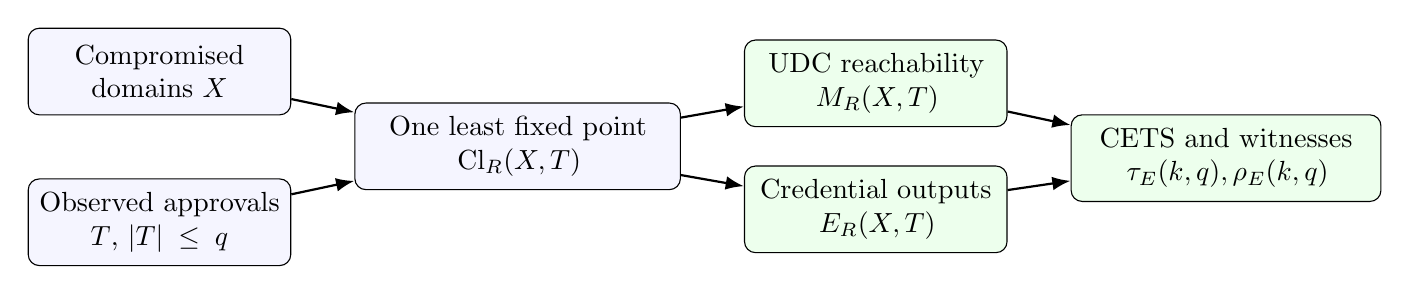
\begin{tikzpicture}[
  node distance=8mm and 8mm,
  box/.style={draw, rounded corners, align=center, minimum height=11mm,
              text width=31mm, fill=blue!4},
  resultbox/.style={draw, rounded corners, align=center, minimum height=11mm,
              text width=31mm, fill=green!7},
  arr/.style={-Latex, thick}
]
\node[box] (domains) {Compromised\\domains $X$};
\node[box, below=of domains] (tickets) {Observed approvals\\$T$, $|T|\le q$};
\node[box, right=of domains, yshift=-9.5mm, text width=39mm] (closure)
  {One least fixed point\\$\operatorname{Cl}_{R}(X,T)$};
\node[resultbox, right=of closure, yshift=8mm] (root)
  {UDC reachability\\$M_R(X,T)$};
\node[resultbox, right=of closure, yshift=-8mm] (exposure)
  {Credential outputs\\$E_R(X,T)$};
\node[resultbox, right=of root, yshift=-9.5mm, text width=37mm] (spectrum)
  {CETS and witnesses\\$\tau_E(k,q),\rho_E(k,q)$};

\draw[arr] (domains) -- (closure);
\draw[arr] (tickets) -- (closure);
\draw[arr] (closure) -- (root);
\draw[arr] (closure) -- (exposure);
\draw[arr] (root) -- (spectrum);
\draw[arr] (exposure) -- (spectrum);
\end{tikzpicture}
}

\caption{A single closure produces UDC reachability and context-indexed
credential exposure; enumeration over $X$ and $T$ produces thresholds and
witnesses.}
\label{fig:pipeline}
\end{figure}

\begin{theorem}[UDC dominance]
\label{thm:root-dominance}
For a well-formed model as defined above,
\[
M_R(X,T)=1\;\Longrightarrow\;E_R(X,T)=C.
\]
\end{theorem}

\begin{proof}
If $M_R(X,T)=1$, the closure contains $\UDC$.  For every $c\in C$, the
well-formedness rule $\{\UDC\}\rightarrow\Derived(c)$ therefore adds
$\Derived(c)$ to the least fixed point.  Thus every $c$ belongs to $E_R(X,T)$;
the reverse inclusion follows from $E_R(X,T)\subseteq C$.
\end{proof}

The theorem rules out a four-independent-quadrant interpretation.
UDC access without output exposure is not a reachable outcome.  The meaningful
distinction appears below the UDC
threshold.

\begin{theorem}[UDC-only incompleteness below threshold]
\label{thm:root-incomplete}
For every finite $C$ with $|C|\ge2$, there exist rule sets $R_1,R_2$ such that
$M_{R_1}(X,T)=M_{R_2}(X,T)=0$ for all $X,T$, while
$E_{R_1}(X,T)\ne E_{R_2}(X,T)$ for some $X,T$.
\end{theorem}

\begin{proof}
Let neither rule set contain a rule producing $\UDC$.  In $R_1$, an honest
evaluator produces a partial evaluation only for the exact context carried by
an observed ticket, giving $E_{R_1}(X,T)=T$ whenever the endpoint interface is
callable.  In $R_2$, the same interface accepts any nonempty observed ticket
for every context, giving $E_{R_2}(X,T)=C$ whenever $T\ne\varnothing$.  The UDC
predicate is identically zero in both systems, but choosing a proper nonempty
$T\subset C$ separates the exposure maps.
\end{proof}

This theorem does not say the two coordinates are independent: by
Theorem~\ref{thm:root-dominance}, $M_R=1$ forces maximal $E_R$.  It says that
the Boolean UDC result loses information precisely in the region where a
DPRF is intended to protect the master.

\section{Credential exposure threshold spectra}

\subsection{Non-amplification and spill}

Let $\mathcal{F}\subseteq\powerset(D)$ be the deployment compromise sets that
the design intends to tolerate.  For an approval budget $q\ge0$, define

\begin{equation}
\mathsf{ACNA}(\mathcal{F},q)\iff
\forall X\in\mathcal{F},\ \forall T\subseteq C,\ |T|\le q:
E_R(X,T)\subseteq T.
\end{equation}

For a particular state, unauthorized spill is
\[
\operatorname{spill}_R(X,T)=|E_R(X,T)\setminus T|.
\]
The maximum spill for fixed $X$ and budget $q$ is
\begin{equation}
A_R(X,q)=\max_{T\subseteq C,\,|T|\le q}
          |E_R(X,T)\setminus T|.
\label{eq:approval-profile}
\end{equation}

\subsection{Cardinality and monotone set-cost spectra}

Let $\Cost:\powerset(D)\rightarrow\mathbb{R}_{\ge0}$ be a compromise-set cost
with $\Cost(\varnothing)=0$ and
$X\subseteq Y\Rightarrow\Cost(X)\le\Cost(Y)$.  This admits correlated
administration, shared tooling, economies of scale, or other coalition costs
that cannot be expressed faithfully by independent per-domain weights.  The
usual additive model $\Cost(X)=\sum_{d\in X}w_d$ is a special case.

\begin{definition}[Credential exposure threshold spectrum]
For target $1\le k\le |C|$ and approval budget $q$, define
\begin{align}
\tau_E(k,q)&=\min\{|X|:\exists T\subseteq C,\ |T|\le q,\
 |E_R(X,T)\setminus T|\ge k\},\label{eq:tau}\\
\rho_E(k,q)&=\min\{\Cost(X):\exists T\subseteq C,\ |T|\le q,\
 |E_R(X,T)\setminus T|\ge k\},\label{eq:rho}
\end{align}
An empty feasible set has value $\infty$.
\end{definition}

The two optimizations are independent.  A single expensive domain may minimize
$\tau_E$, while a larger coalition with a lower modeled set cost may minimize
$\rho_E$.  Reporting only the cost of the cardinality-minimal witness would not
compute Eq.~\eqref{eq:rho}.  Monotonicity of $\Cost$ prevents adding compromised
domains from making an attack cheaper, but additivity is not required.

\begin{proposition}[Spectrum monotonicity]
For fixed $q$, $\tau_E(k+1,q)\ge\tau_E(k,q)$ and
$\rho_E(k+1,q)\ge\rho_E(k,q)$.  For fixed $k$, both values are nonincreasing as
$q$ increases.
\end{proposition}

\begin{proof}
A witness exposing at least $k+1$ unauthorized contexts also exposes at least
$k$, so the feasible set for $k+1$ is contained in that for $k$.  Conversely,
the constraint $|T|\le q$ defines a subset of the feasible ticket sets for
$q+1$.  Taking minima gives the stated inequalities.
\end{proof}

Define the ticket-free UDC threshold
\[
\tau_M^{0}=\min\{|X|:M_R(X,\varnothing)=1\}
\]
and its set-cost analogue $\rho_M^{0}$.  Ticket-free is explicit because a
recovery design might otherwise use approvals as premises for UDC release.

\begin{corollary}[UDC bound]
Under Theorem~\ref{thm:root-dominance}, for every $q\ge0$ and
$1\le k\le|C|$,
\[
\tau_E(k,q)\le\tau_M^{0},\qquad
\rho_E(k,q)\le\rho_M^{0}.
\]
\end{corollary}

\begin{proof}
A minimum ticket-free UDC witness $X$ is feasible for the spectrum because
$T=\varnothing$ satisfies every upper budget $q$.  UDC dominance gives
$E_R(X,\varnothing)=C$, so spill is $|C|$.
\end{proof}

The inequality can be strict.  An over-broad evaluator may expose $k<|C|$
outputs after one endpoint compromise even when two domains are required for
UDC.

\section{Projection-bound authorization}

Many implementations do not express an arbitrary predicate over $C$; they
compare selected ticket fields.  Let $B$ be a subset of the canonical fields
and let $\pi_B(c)$ be their ordered projection.  A ticket for $c$ is accepted
for $c'$ exactly when $\pi_B(c')=\pi_B(c)$.  This partitions $C$ into
equivalence classes
\[
[c]_B=\{c'\in C:\pi_B(c')=\pi_B(c)\}.
\]

\begin{theorem}[Projection-exposure identity]
\label{thm:projection}
Assume a compromised endpoint can request every context and compute its own
partial evaluation, while an honest participant returns its partial exactly
when the ticket projection matches.  For a single ticket authorizing $c$ and
without UDC access,
\[
E_R(X,\{c\})=[c]_B.
\]
\end{theorem}

\begin{proof}
Every $c'\in[c]_B$ passes the honest participant's only authorization predicate;
the endpoint supplies the other partial, so $\Derived(c')$ is in the closure.
Every $c'\notin[c]_B$ fails that predicate, and by assumption no other rule
produces the missing partial or UDC.  Hence it cannot enter
$E_R$.
\end{proof}

\begin{corollary}[Injectivity criterion]
In the profile of Theorem~\ref{thm:projection}, exact one-context
non-amplification holds for all $c\in C$ iff $\pi_B$ is injective on $C$.
\end{corollary}

Injectivity over the current finite database is not a future-proof protocol
condition.  A deployable ticket should bind a collision-resistant digest of
the complete canonical derivation context, the operation identifier, expiry,
freshness generation, and protocol version.  The digest must be computed from
an unambiguous encoding.

\begin{theorem}[Exact approval-budget profile]
\label{thm:budget-profile}
Let the projection partition have class sizes
$s_1\ge s_2\ge\cdots\ge s_p$.  Under the assumptions of
Theorem~\ref{thm:projection},
\[
A_R(X,q)=\sum_{i=1}^{\min(q,p)}(s_i-1).
\]
\end{theorem}

\begin{proof}
The first ticket in a class exposes its other $s_i-1$ members.  A further
ticket in that class cannot add an exposed context and moves one already
exposed context into the approved set, so it cannot improve the objective.
An optimum therefore selects at most one member per class and selects the
largest class gains first.
\end{proof}

This closed form is specific to equality on a projection.  General rule sets
still require closure enumeration or a more scalable symbolic engine.

\section{Reference analysis algorithm}

The reference implementation intentionally supports a small two-layer subset
of the semantics: unparameterized deployment-capability rules are followed by
an exact, wildcard, or field-projection evaluator for context-indexed outputs.
It uses exhaustive enumeration and is appropriate when the number of
operational trust domains and the approval budget are small.

For every $X\subseteq D$, it computes the deployment closure by repeatedly
applying enabled monotone rules. It then enumerates every $T\subseteq C$ with
$|T|\le q$, applies the selected evaluator semantics, and records
$M_R(X,T)$, $E_R(X,T)$, spill, and a supplied $\Cost(X)$.  The library API
accepts any finite monotone set-cost oracle and validates monotonicity by
enumeration; the command-line reference models use additive domain weights.
For each $k$, it separately updates:

\begin{enumerate}[leftmargin=*]
\item the lexicographically best cardinality witness
  $(|X|,\Cost(X))$ for $\tau_E(k,q)$; and
\item the lexicographically best set-cost witness
  $(\Cost(X),|X|)$ for $\rho_E(k,q)$.
\end{enumerate}

Minimal UDC witnesses are reduced by set inclusion.  Exposure witnesses retain
the compromised domains, approved context indexes, cause classification, and
whether UDC was reachable.

\begin{proposition}[Reference-algorithm exactness]
For finite $D,C,K$, monotone deployment rules, a supported evaluator mode, and
budget $q$, the exhaustive reference algorithm returns
Eqs.~\eqref{eq:tau}--\eqref{eq:rho} exactly for that encoded model.
\end{proposition}

\begin{proof}
The algorithm enumerates every feasible $X$ and $T$. Fixed-point iteration is
sound because it adds only deployment-rule consequences and complete because it
stops only when no enabled consequence remains. The selected evaluator then
computes exactly the exposure set defined for its mode. Each feasible spill is
therefore visited, and independent minima over all visited witnesses equal the
defining minima.
\end{proof}

With $d=|D|$ and $n=|C|$, the number of analyzed pairs is
\[
2^d\sum_{i=0}^{q}\binom{n}{i}.
\]
If closure evaluation costs $L$, the direct bound is
$O(d2^d+2^d\sum_{i=0}^{q}\binom{n}{i}(L+n))$, including monotonicity checks
along every edge of the subset lattice for an externally supplied cost oracle.
This is not proposed as a new generic attack-graph algorithm.  Production-scale
models can reuse symbolic or Datalog engines while preserving the same output
definitions.

\section{Evaluation}

\subsection{Research questions and method}

The evaluation asks:

\begin{description}[leftmargin=14mm,style=nextline]
\item[RQ1] Does CETS distinguish deployments with the same UDC threshold but
different callable-output exposure?
\item[RQ2] Does the projection identity predict exposure as context fields are
bound?
\item[RQ3] Do the predicted exposure sets persist in a complete scoped
credential-key derivation protocol rather than only a symbolic evaluator?
\item[RQ4] What is the local cost of the standalone projection analyzer and
the complete reference scoped key-derivation path?
\item[RQ5] Does a temporal state model preserve scope across ticket issue,
expiry, revocation, replay, and generation change?
\end{description}

The controlled context space is the Cartesian product of five binary fields:
service, account, credential lineage, Root generation, and policy identity,
giving 32 contexts.  These configurations isolate semantics; they are not
encodings of, or security claims about, the published systems in
Section~2.

We model six deployment patterns around a nominal 2-of-3 recovery structure:
automatic network release; independent approval; approval authority colocated
with the endpoint; a release credential colocated with removable media; a
3-of-5 network layer entirely callable by one endpoint; and three network
fragments plus approval in one administrative domain.  Domain compromise costs
are explicit test parameters, not empirical probabilities.

The analyzer tests ran with Python~3.  The reference protocol was compiled in
release mode with Rust 1.87 on macOS 26.5.2 and an Intel Core i9-9880H.  Timing
reports the median and nearest-rank P95.  Projection-analyzer timing excludes
network, storage, ticket issuance, and cryptographic evaluation; reference
protocol timing is reported separately.

\subsection{Deployment threshold results}

Table~\ref{tab:deployments} shows that only the independent-approval pattern
preserves the configured two-domain threshold.  Additional nodes do not help
when one endpoint capability can automatically invoke enough of them; physical
node count is not an access structure over compromise domains.

\begin{table}[t]
\centering
\caption{Controlled deployment-pattern analysis.}
\label{tab:deployments}
\small
\begin{tabularx}{\textwidth}{Y c c Y}
\toprule
Pattern & Configured $t$ & Effective $t$ & Minimum witness characteristic \\
\midrule
Automatic network release & 2 & 1 & Endpoint calls honest release \\
Independent approval & 2 & 2 & Two independently controlled domains \\
Approval authority at endpoint & 2 & 1 & Endpoint owns request and approval \\
Release credential on removable medium & 2 & 1 & Medium invokes network release \\
3-of-5 nodes callable by endpoint & 2 & 1 & One token drives three node fragments \\
Shared administrative domain & 2 & 1 & One administration boundary holds endpoint, approval, and fragments \\
\bottomrule
\end{tabularx}
\end{table}

\subsection{Spectra distinguish the missing failure}

We combine two access patterns with exact and unscoped evaluation interfaces.
The resulting analytical cases are:

\begin{enumerate}[leftmargin=*]
\item independent approval, UDC threshold two, exact context binding;
\item the same UDC threshold, but one callable unscoped interface; and
\item a collapsed one-domain UDC threshold with exact ticket binding.
\end{enumerate}

For a one-ticket budget, their cardinality spectra are respectively
\[
[2,\ldots,2],\qquad [\underbrace{1,\ldots,1}_{31},2],\qquad
[1,\ldots,1].
\]
The second case passes a UDC-only threshold check but one compromised endpoint
exposes any target up to 31 unauthorized contexts.  Exposing all 32 is different
because one approved context is excluded from spill; the ticket-free UDC
witness supplies the final spectrum point at threshold two.  Figure
\ref{fig:spectra} shows the curves.

\begin{figure}[t]
\centering
\resizebox{0.98\linewidth}{!}{%
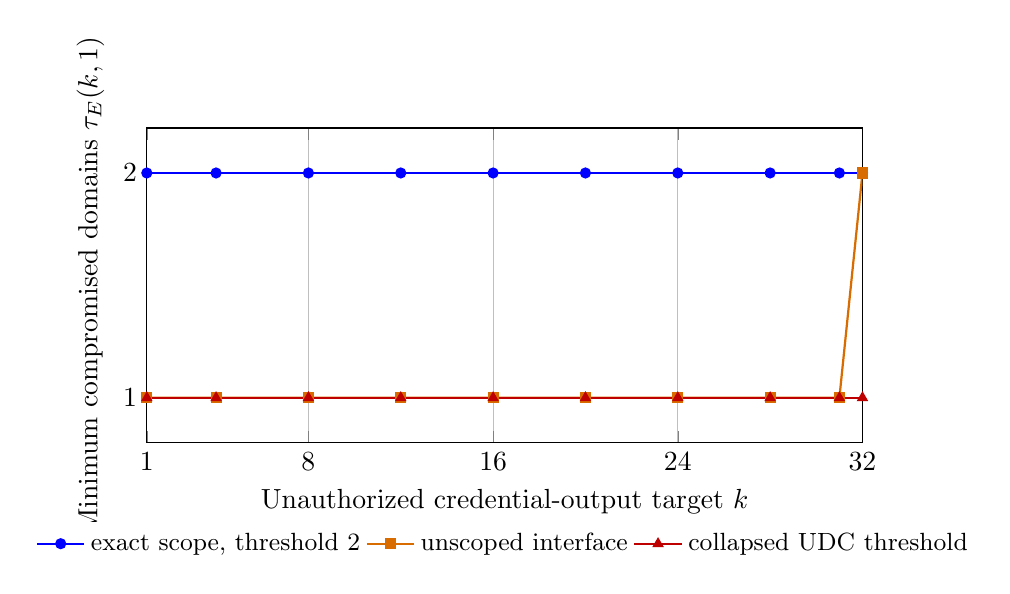
\begin{tikzpicture}
\begin{axis}[
  width=0.88\linewidth,
  height=0.46\linewidth,
  xlabel={Unauthorized credential-output target $k$},
  ylabel={Minimum compromised domains $\tau_E(k,1)$},
  xmin=1, xmax=32,
  ymin=0.8, ymax=2.2,
  xtick={1,8,16,24,32},
  ytick={1,2},
  grid=major,
  legend style={font=\small, at={(0.5,-0.25)}, anchor=north,
                legend columns=3, draw=none},
  mark size=1.6pt
]
\addplot[blue, thick, mark=*] coordinates {
 (1,2) (4,2) (8,2) (12,2) (16,2) (20,2) (24,2) (28,2) (31,2) (32,2)};
\addlegendentry{exact scope, threshold 2}
\addplot[orange!85!black, thick, mark=square*] coordinates {
 (1,1) (4,1) (8,1) (12,1) (16,1) (20,1) (24,1) (28,1) (31,1) (32,2)};
\addlegendentry{unscoped interface}
\addplot[red!75!black, thick, mark=triangle*] coordinates {
 (1,1) (4,1) (8,1) (12,1) (16,1) (20,1) (24,1) (28,1) (31,1) (32,1)};
\addlegendentry{collapsed UDC threshold}
\end{axis}
\end{tikzpicture}
}

\caption{Credential exposure threshold spectra for three controlled
configurations over 32 contexts and approval budget one.}
\label{fig:spectra}
\end{figure}

The dual Boolean summaries are $(0,0)$, $(0,1)$, and $(1,1)$ for, respectively,
no collapse, scope amplification below the UDC threshold, and UDC-threshold
collapse.  The absent $(1,0)$ outcome agrees with
Theorem~\ref{thm:root-dominance}.

\subsection{Context-binding curve}

Table~\ref{tab:binding} binds fields cumulatively.  Because each omitted binary
field doubles a projection equivalence class, the measured exposure equals the
closed form exactly.  The unscoped interface and Root reconstruction (an
instance of UDC) both
expose 32 outputs, demonstrating that master non-materialization alone does not
reduce worst-case callable-output exposure.

\begin{table}[t]
\centering
\caption{Single-ticket exposure over the 32-context factorial space.}
\label{tab:binding}
\small
\begin{tabular}{lrr}
\toprule
Evaluator or bound fields & Exposed contexts & Unauthorized spill \\
\midrule
UDC via Root reconstruction & 32 & 31 \\
Unscoped DPRF interface & 32 & 31 \\
Service & 16 & 15 \\
Service, account & 8 & 7 \\
$+$ lineage & 4 & 3 \\
$+$ Root generation & 2 & 1 \\
$+$ policy identity & 1 & 0 \\
\bottomrule
\end{tabular}
\end{table}

Approval budgets reveal structure that one ticket does not.  Service-only
binding creates two classes of size 16, so Eq.~\eqref{eq:approval-profile} gives
maximum spill $[15,30,30,30]$ for budgets one through four.  Full binding gives
32 singleton classes and $[0,0,0,0]$.

\subsection{Cryptographic reference protocol}
\label{sec:reference-protocol}

To test that the symbolic result survives a complete scoped credential-key
derivation path, we built the two-server reference protocol in
Figure~\ref{fig:poprf-sequence}.  It uses
the RFC~9497 POPRF mode with the ristretto255-SHA512 ciphersuite
\cite{rfc9497}.  Evaluators A and B hold independent POPRF keys.  The client
samples one stable 32-byte input $x$ for the reference run and uses that same
input for every configured context.  In the threat model, a compromised
endpoint obtains $x$ and all candidate contexts; $x$ is therefore not an
additional authorization boundary.  POPRF blinding treats it as private from
either evaluator in the protocol transcript.  With the complete canonical
context supplied as POPRF public information, the client obtains and verifies
\[
Y_A=\mathsf{POPRF}_{k_A}(x;\mathsf{Canon}(c)),\qquad
Y_B=\mathsf{POPRF}_{k_B}(x;\mathsf{Canon}(c)),
\]
then computes
\[
K_c=H(\mathtt{cets\mbox{-}combined\mbox{-}v1}\parallel
Y_A\parallel Y_B\parallel\mathsf{Canon}(c)).
\]
$K_c$ is a credential-specific secret consumed by a downstream deterministic
password encoder; character-policy encoding is orthogonal to CETS and is not
evaluated here.  Both POPRF outputs are necessary.  The minimum UDC witness in
this deployment is compromise of the endpoint together with the approval
authority: the former supplies $x$ and arbitrary candidate contexts, while the
latter can mint valid tickets that the two honest evaluators accept.  A
separate path compromises the endpoint and both evaluator domains.  The first
path has two domains, the second has three, and the evaluator pair alone lacks
$x$.  Consequently, the effective UDC threshold is two.  This is a conjunctive
composition of two published POPRF instances, not a claim to a new
threshold-shared PRF.

For a configured binding-field set $B$, define
\[
d_B(c)=H(\mathtt{cets\mbox{-}ticket\mbox{-}binding\mbox{-}v1}\parallel
          \mathsf{Canon}(\pi_B(c))).
\]
The exact configuration selects all five fields; the projected configuration
selects only service and account; and the wildcard configuration sets
$B=\varnothing$.  An independent Ed25519 authority signs the protocol version,
operation, the identifier of $B$, $d_B(c)$, issue and expiry epochs, freshness
generation, and nonce.  Each evaluator verifies the signature, requires the
signed $B$ to equal its configured binding set, and checks the remaining state
fields before evaluation.  In
all configurations, POPRF public information is the \emph{complete} canonical
context; only the application verifier is varied.  The exact verifier compares
a digest of all five fields, the projected verifier compares service and
account only, and the wildcard negative control ignores context identity.
The reference prototype intentionally reuses one still-live ticket to measure
its accepted context set; it does not implement durable nonce-use or revocation
storage.  Section~\ref{sec:tla-evaluation} analyzes those temporal controls
separately.

\begin{figure}[t]
\centering
\resizebox{\textwidth}{!}{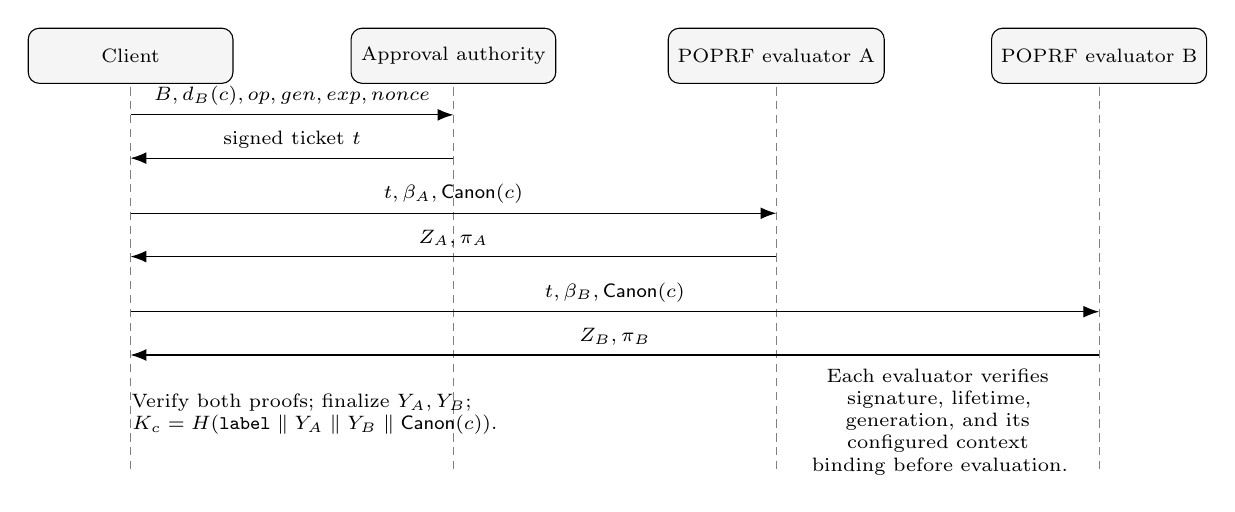
\begin{tikzpicture}[
  actor/.style={draw,rounded corners,fill=gray!8,minimum width=26mm,minimum height=7mm,font=\scriptsize},
  msg/.style={-{Latex[length=2mm]},thin},
  every node/.style={font=\scriptsize}
]
\node[actor] (client) at (0,0) {Client};
\node[actor] (approval) at (4.1,0) {Approval authority};
\node[actor] (evala) at (8.2,0) {POPRF evaluator A};
\node[actor] (evalb) at (12.3,0) {POPRF evaluator B};

\foreach \x in {0,4.1,8.2,12.3}
  \draw[densely dashed,gray] (\x,-0.4) -- (\x,-5.25);

\draw[msg] (0,-0.75) -- node[above] {$B,d_B(c),op,gen,exp,nonce$} (4.1,-0.75);
\draw[msg] (4.1,-1.3) -- node[above] {signed ticket $t$} (0,-1.3);
\draw[msg] (0,-2.0) -- node[above] {$t,\beta_A,\mathsf{Canon}(c)$} (8.2,-2.0);
\draw[msg] (8.2,-2.55) -- node[above] {$Z_A,\pi_A$} (0,-2.55);
\draw[msg] (0,-3.25) -- node[above] {$t,\beta_B,\mathsf{Canon}(c)$} (12.3,-3.25);
\draw[msg] (12.3,-3.8) -- node[above] {$Z_B,\pi_B$} (0,-3.8);

\node[align=left,anchor=west,text width=47mm] at (-0.1,-4.55)
  {Verify both proofs; finalize $Y_A,Y_B$;\\
   $K_c=H(\mathtt{label}\parallel Y_A\parallel Y_B\parallel\mathsf{Canon}(c))$.};
\node[align=center,text width=34mm] at (10.25,-4.65)
  {Each evaluator verifies signature, lifetime, generation, and its configured context binding before evaluation.};
\end{tikzpicture}
}
\caption{Complete two-server POPRF scoped credential-key derivation.  The
ticket-binding predicate is evaluated independently by both servers before the
standardized cryptographic operation.}
\label{fig:poprf-sequence}
\end{figure}

Table~\ref{tab:poprf-results} reports actual ticket verification, POPRF blind
evaluation, proof verification, finalization, and output combination for every
context.  The accepted-set sizes equal the projection theorem: 1, 8, and 32.
Repeated evaluation of one context was deterministic; all 32 context outputs
were distinct in this finite sample; and a post-signature ticket mutation was
rejected.  These checks are functional evidence, not a collision-resistance
estimate.

\begin{table}[t]
\centering
\caption{Two-server RFC~9497 POPRF reference protocol, one signed ticket and
32 candidate contexts.}
\label{tab:poprf-results}
\small
\begin{tabularx}{\textwidth}{Y r r Y}
\toprule
Ticket binding & Accepted & Spill & CETS for $q=1$ \\
\midrule
Complete five-field context & 1 & 0 & $2$ for every $k$ \\
Service and account only & 8 & 7 & $1$ for $k\le7$; $2$ otherwise \\
Wildcard negative control & 32 & 31 & $1$ for $k\le31$; $2$ for $k=32$ \\
\bottomrule
\end{tabularx}
\end{table}

The threshold value two in Table~\ref{tab:poprf-results} is induced by the
minimum UDC witness $\{\text{endpoint},\text{approval authority}\}$; the two
evaluator domains alone are not a witness.

Across 1,000 complete exact-scope credential-key derivations, local latency was
1.151~ms median and 1.456~ms P95.  This includes two POPRF proof flows and
ticket verification, but excludes network round trips, approval
delay, and durable replay storage.  It is a cryptographic baseline rather than
a production-service latency claim.

\subsection{Local analysis cost}

Table~\ref{tab:performance} reports the standalone projection analyzer.  The
observed scaling is approximately linear for a fixed field projection, as
expected from one pass that constructs projection classes.  The 100,000-context
median is 3.56~s.  This is an offline analysis-tool measurement, not credential
derivation latency.

\begin{table}[t]
\centering
\caption{Local projection-analysis latency over five runs.}
\label{tab:performance}
\small
\begin{tabular}{rrr}
\toprule
Contexts & Median (ms) & P95 (ms) \\
\midrule
32 & 1.40 & 1.55 \\
1,024 & 34.82 & 36.88 \\
10,000 & 335.01 & 340.12 \\
100,000 & 3,555.38 & 3,863.90 \\
\bottomrule
\end{tabular}
\end{table}

\subsection{Tests and temporal model checking}
\label{sec:tla-evaluation}

Twenty Python tests cover closure witnesses, deployment thresholds, projection
classes, approval-budget profiles, the three reachable dual outcomes,
cardinality spectra, independent set-cost minimization, and rejection of a
non-monotone cost oracle.  Four Rust tests cover canonical encoding, the three
ticket-scope cardinalities, output determinism and context separation, and
signature/lifetime enforcement.

The TLA+ model \cite{lamport2002tla} has two credential contexts, time values
$0..2$, and two freshness generations.  Its state records ticket issue,
expiry, revocation, use count, derivation requests, partial evaluations, an
abstract UDC flag, and exposed outputs.
Evaluators check exact scope, ticket
lifetime, revocation state, freshness generation, and single use.  The model
also permits UDC acquisition and checks that it immediately exposes all
contexts.  This action abstracts deployment-specific witnesses; in the
reference interpretation it represents either endpoint-plus-approval
compromise or the endpoint-plus-both-evaluators path, never the evaluator pair
alone.

With every control enabled, TLC exhaustively generated 3,997 states and 888
distinct states, reached graph depth 10, and left no states on the queue.  The
type, UDC-dominance, below-UDC scope, expiry, revocation, generation, and
replay invariants all held.  Five single-fault configurations provide negative
controls.  A projected-context verifier reaches the expected cross-context
exposure trace; disabling expiry, revocation, generation, or single-use checks
reaches the corresponding expired-ticket, revoked-ticket, stale-generation,
or replay acceptance trace.  Thus each asserted temporal control is exercised
by a concrete counterexample when removed.  We do not compare generated-state
counts for fault models because parallel TLC may discover the same
counterexample after different amounts of frontier work.

These finite exhaustive checks validate the final abstract transition
relation and its control dependencies.  They do not verify the POPRF library,
hardware isolation, durable storage, network liveness, or unbounded time.

\section{Security interpretation and repair}

\subsection{Two necessary controls}

The results imply that threshold preservation and exact evaluation scoping are
both necessary for compartmentalization:

\begin{enumerate}[leftmargin=*]
\item Deployment shares, request credentials, approval keys, and network
  participants must be assigned to actual compromise domains.  An honest
  service that automatically releases a qualifying capability to a compromised
  endpoint can collapse the effective threshold without being compromised.
\item Every partial evaluator must validate the complete canonical derivation
  context and the intended operation.  A secure DPRF with an unscoped
  application interface can preserve its master-key theorem while exposing
  legitimate outputs on attacker-chosen inputs.
\end{enumerate}

These controls are conjunctive.  Exact tickets do not repair UDC compromise;
additional shares do not repair an over-broad evaluation oracle.

\subsection{Binding construction boundary}

A practical approval can use the domain-separated projection digest $d_B(c)$
defined in Section~\ref{sec:reference-protocol} and sign or MAC an unambiguous
encoding of
\[
\begin{aligned}
&\mathsf{protocolVersion}\parallel\mathsf{operation}\parallel
  B\parallel d_B(c)\parallel{}\\
&\mathsf{freshness}\parallel\mathsf{expiry}\parallel\mathsf{nonce}.
\end{aligned}
\]
For a production non-amplifying interface, $B$ contains the complete canonical
derivation context; proper subsets are the analyzed projection cases.
Collision resistance, signature or MAC unforgeability, replay control, and
canonical encoding are required.  Existing contextual capabilities and
constrained PRFs provide construction options
\cite{birgisson2014macaroons,boneh2013constrained}.  CETS decides whether the
resulting interface amplifies the modeled approvals; it does not replace the
underlying security proof.

\subsection{Conditional composition statement}

Suppose a reviewed DPRF is secure for the chosen corruption model under
adaptive queries; fewer than its threshold parties reveal no master key; ticket
verification is unforgeable and binds the complete canonical context; the
protocol satisfies $\mathsf{ACNA}(\mathcal{F},q)$; and no other closure rule
releases a raw share or UDC.  Then, for $X\in\mathcal{F}$ and
$c^*\notin T$, the application provides no authorized evaluation path for
$c^*$.  The adversary's remaining ability to distinguish or compute the fresh
output reduces to the selected DPRF advantage, ticket-forgery probability, and
context-digest collision probability.

This is a composition boundary, not a new DPRF theorem.  Its purpose is to make
the authorization premise explicit rather than silently importing it into a
master-key security claim.

\section{Limitations and validity}

\paragraph{Finite monotone semantics}
The spectrum analyzer does not natively represent revocation, time, rate
limits, probabilities, concurrency, or non-monotone state.  A short-lived
ticket is modeled only as present or absent in one analysis epoch.  The
separate temporal model covers bounded issue, expiry, revocation, replay, and
generation transitions, but not unbounded executions or probabilistic events.

\paragraph{Model fidelity}
Results are only as sound as domain boundaries, automatic-rule classification,
and context canonicalization.  Administrative correlation can invalidate a
claimed independent domain.  Conversely, placing all legitimate approvals in
$T$ would overstate attacker authority.  Independent model review is required
for claims about a concrete system.

\paragraph{Evidence scope}
The deployment configurations are controlled models designed to exercise the
definitions.  The POPRF case is an executable scoped key-derivation reference
protocol, but
it is not an independently reviewed encoding of a published end-to-end system
or a production deployment.  Analyzer timing and local cryptographic timing
exclude network, storage, and human approval delay and should not be read as
end-to-end service performance.

\paragraph{Cryptographic boundary}
The reference case invokes a published POPRF implementation and verifies its
proofs; it neither proves that library nor implements a threshold-shared single
PRF key.  Its conjunctive two-key composition is a case-study mechanism, not a
new primitive.  Adaptive multi-server corruption, availability under a
malicious evaluator, side channels, durable replay-state failure, and key
erasure require separate treatment.  A fully compromised endpoint during a
legitimate password-use session can observe that password.

\paragraph{Novelty boundary}
The phrase CETS names the metric defined here; it is not evidence of worldwide
priority.  Fixed-point reachability, minimum-cost attack analysis, authority
safety, permission expansion, scoped authorization, and DPRFs are established
work.  The defensible contribution is their credential-specific joint output,
UDC relation, and approval-budget-indexed exposure curve.

\section{Conclusion}

A UDC threshold answers when a deterministic credential hierarchy is wholly
compromised, but not how many legitimate outputs can be obtained through a
callable interface before that threshold is reached.  The proposed semantics
computes both facts from one capability closure.  UDC dominance removes an
invalid independent-failure state; UDC-only incompleteness shows why the
remaining below-threshold region needs a set-valued output analysis.  CETS then
turns that set into cardinality and cost curves indexed by the approval budget.
The cost coordinate permits any monotone compromise-set cost, retaining
additive weights only as a convenient reference instance.

For projection-bound tickets, exposure is exactly an equivalence class and the
multi-ticket spill has a closed form.  In the executable POPRF case, complete,
service/account, and wildcard binding accept 1, 8, and 32 of 32 candidate
contexts, producing exactly the predicted spectra.  The temporal model further
shows that scope must be combined with expiry, revocation, replay, and
generation checks.  The resulting design test is concise: protect both the
UDC and the authority to request each credential output throughout
the ticket lifecycle.

\appendix

\section{Reproducibility boundary}

The accompanying artifact contains:

\begin{itemize}[leftmargin=*]
\item JSON models for six deployment patterns, seven context-binding patterns,
  and three joint cases;
\item a standard-library Python closure and spectrum analyzer;
\item a Rust two-server RFC~9497 POPRF reference protocol, dependency lockfile,
  signed-ticket checks, and generated JSON results;
\item generated JSON witnesses and local scaling results;
\item 20 Python tests and 4 Rust tests; and
\item the temporal TLA+ model and six configurations summarized in
  Section~\ref{sec:tla-evaluation}.
\end{itemize}

The artifact is intended to reproduce the finite claims in this paper.  It is
not a production credential service, cryptographic library, or certification of
any cited published system.

\bibliographystyle{elsarticle-num}
\bibliography{references}

\end{document}
